This is some data we had:

\begin{Schunk}
\begin{Sinput}
> z=read.table("z.txt",header=T)
> attach(z)
> x
\end{Sinput}
\begin{Soutput}
 [1] -0.07943649 -0.18656098 -0.44115429  1.76839347  0.61555461  0.88498442
 [7]  0.99487305 -0.62048182 -0.30419035  1.55566471  0.84008788 -0.13675295
[13] -0.66324285 -0.04459009  0.34443517 -0.30036085  1.64238151  0.12964675
[19]  0.26278791  0.98366936
\end{Soutput}
\begin{Sinput}
> y
\end{Sinput}
\begin{Soutput}
 [1] -0.02808897  0.39538936 -0.10344437 -0.80405243  0.76664016  0.78937257
 [7]  1.38315206 -3.24039716 -0.77773418 -1.25822706  0.01332692 -1.18757644
[13]  0.26308404 -0.17699518  0.54277135  2.43535887  0.18996337 -1.96440864
[19] -0.14357622  1.35470342
\end{Soutput}
\end{Schunk}


Here is a scatterplot of it:

\begin{Schunk}
\begin{Sinput}
> plot(y~x)
\end{Sinput}
\end{Schunk}
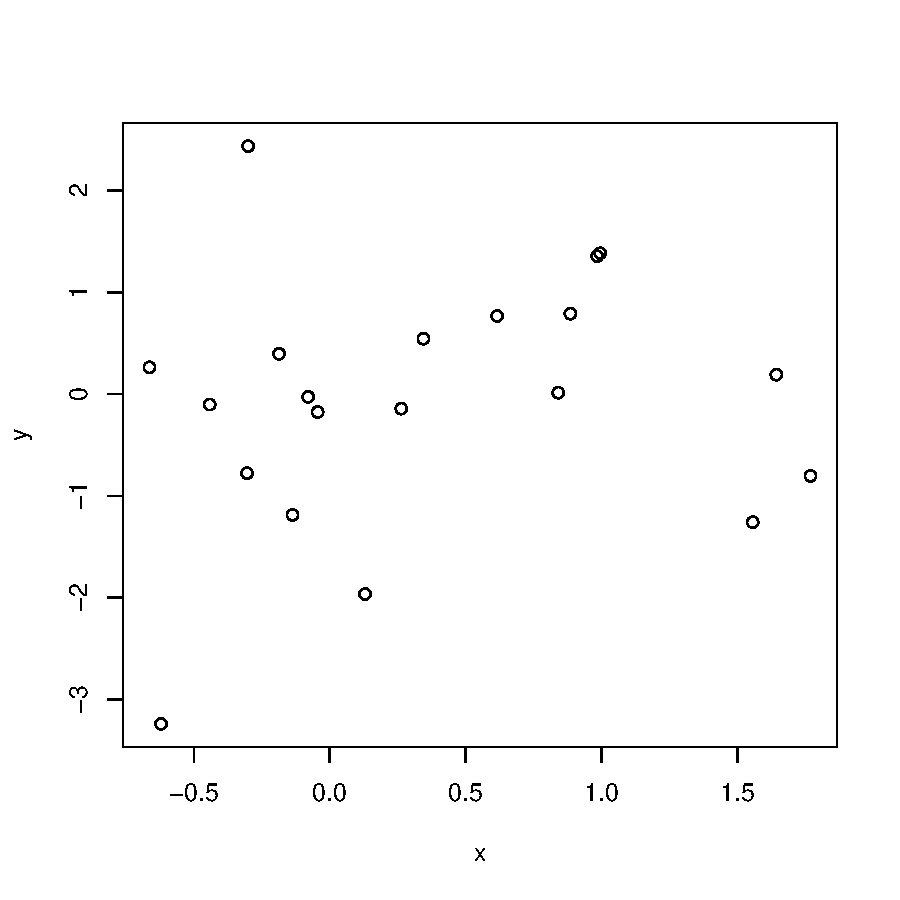
\includegraphics{second-002}
